%!TEX root = ../Thesis.tex
\chapter{Service Requirements for Aggregators} % (fold)
\label{cha:services}
\begin{marginfigure}
	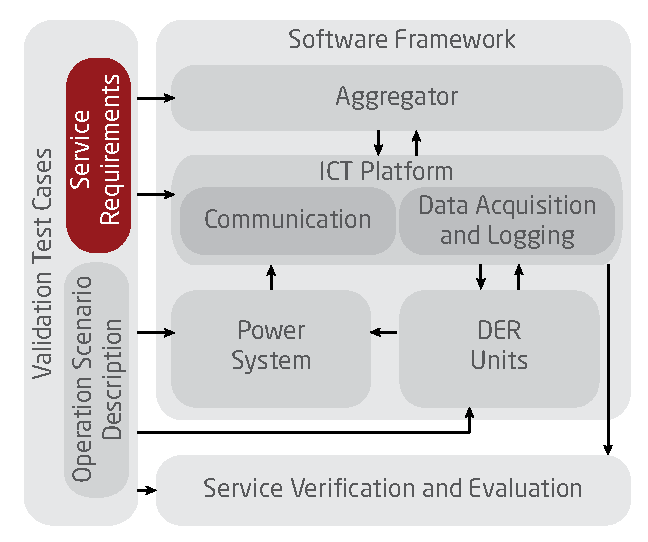
\includegraphics[width=\textwidth]{framework_services.eps}
	\caption{This chapter focuses on the \emph{service definition} block of the aggregator validation framework presented in Chapter~\ref{cha:validation}.}
      \label{fig:frameworkservices}
\end{marginfigure}
\newchapter{I}{t is clear from} Chapter~\ref{cha:validation} that \emph{service requirements} is an essential block in the aggregator validation framework (see Figure~\ref{fig:frameworkservices}). Initially, an objective of this work was to model service requirements in order to perform the aggregator validation. While this objective was achieved, it is clear that current service requirements in many countries are directly, or indirectly, blocking the integration of aggregators providing DR\fcite{cappers2013assessment,coalition2014mapping}. If aggregators are to be successfully integrated into the power system, the rules and requirements for participation must be changed. This chapter presents two novel contributions to integrating aggregators in the power system: a modeling method for ancillary services, and a proposal for the restructuring of requirements for ancillary services. A method for modeling ancillary services is important because the resulting models form the benchmark for the performance evaluation and verification of the aggregator, as well as being a direct input to the aggregator (as discussed in Chapter~\ref{cha:aggregator}). The redefinition of ancillary service requirements is important since it will allow system operators to utilize the properties of all available resources, both traditional and new, in an optimal way.

The service modeling method is part of a submitted journal paper\fcite{bondy2016method} and the requirements restructuring is part of a draft journal paper\fcite{bondy2016redefining}. This draft journal paper is the outcome of my external research stay.

%Content of this chapter is the work done at LBNL and through the iPower demo.
%\begin{itemize}
%	\item Service definition
%	\item What are aggregators expected to deliver?
%	\item PowerMax service requirements
%	\item Redefining Ancillary Services Requirements for Technology Agnostic Resources
%\end{itemize}

Aggregators/DR provide flexibility, as it is, they are not being paid for flexibility as defined previously, but only for power. This needs rethinking.
\section{Background} % (fold)
\label{sec:backgroundservices}
\subsection{Service Requirements for Ancillary Services} % (fold)
\label{sub:servreqAS}

% subsection Service Requirements for Ancillary Services (end)
\subsection{Demand as Ancillary Services} % (fold)
\label{sub:demandAS}
The concept of using demand side management to help the secure operation of the power grid has existed in different forms since the late 1970s\fcite{lampropoulos2013history}. But in recent years, the introduction of new consumption and generation technologies, \ie DERs, along with the roll-out of a smart metering infrastructure and the advances in ICT, has lead to the new opportunities in using smart control of consumption as a service to the power grid. 

The 
% subsection Demand as Ancillary Services (end)

% section Background on Aggregator Services (end)
\section{Modeling of Ancillary Services} % (fold)
\label{sec:Modeling of Ancillary Services}

% section Modeling of Ancillary Services (end)

\section{Redefining Ancillary Service Requirements} % (fold)
\label{sec:Redefining Ancillary Service Requirements}

% section Redefining Ancillary Service Requirements (end)
% chapter Service Requirements (end)

